% Provenance (never printed): cycle 2 "Questionner le monde" (states of water in
% weather phenomena; daily observation), see sources/book1/PROVENANCE.md.
% Book 1, grade 1, chapter 1. No real-world number in this chapter.
\chapter{观察天气}\label{ch:g1:watching-the-weather}

早晨到了。莉娜醒来，爬上卧室窗前的椅子，
朝外看。天空灰蒙蒙的。小水滴
顺着玻璃往下流。街对面的屋顶湿漉漉、亮晶晶的，花园里的
树正在滴水。

“我今天穿什么呢？”她问。

要回答这个问题，莉娜不需要书，也不需要仪器。她只需
朝窗外看一看。这扇窗户就是她的第一个气象站。

\begin{omfigure}
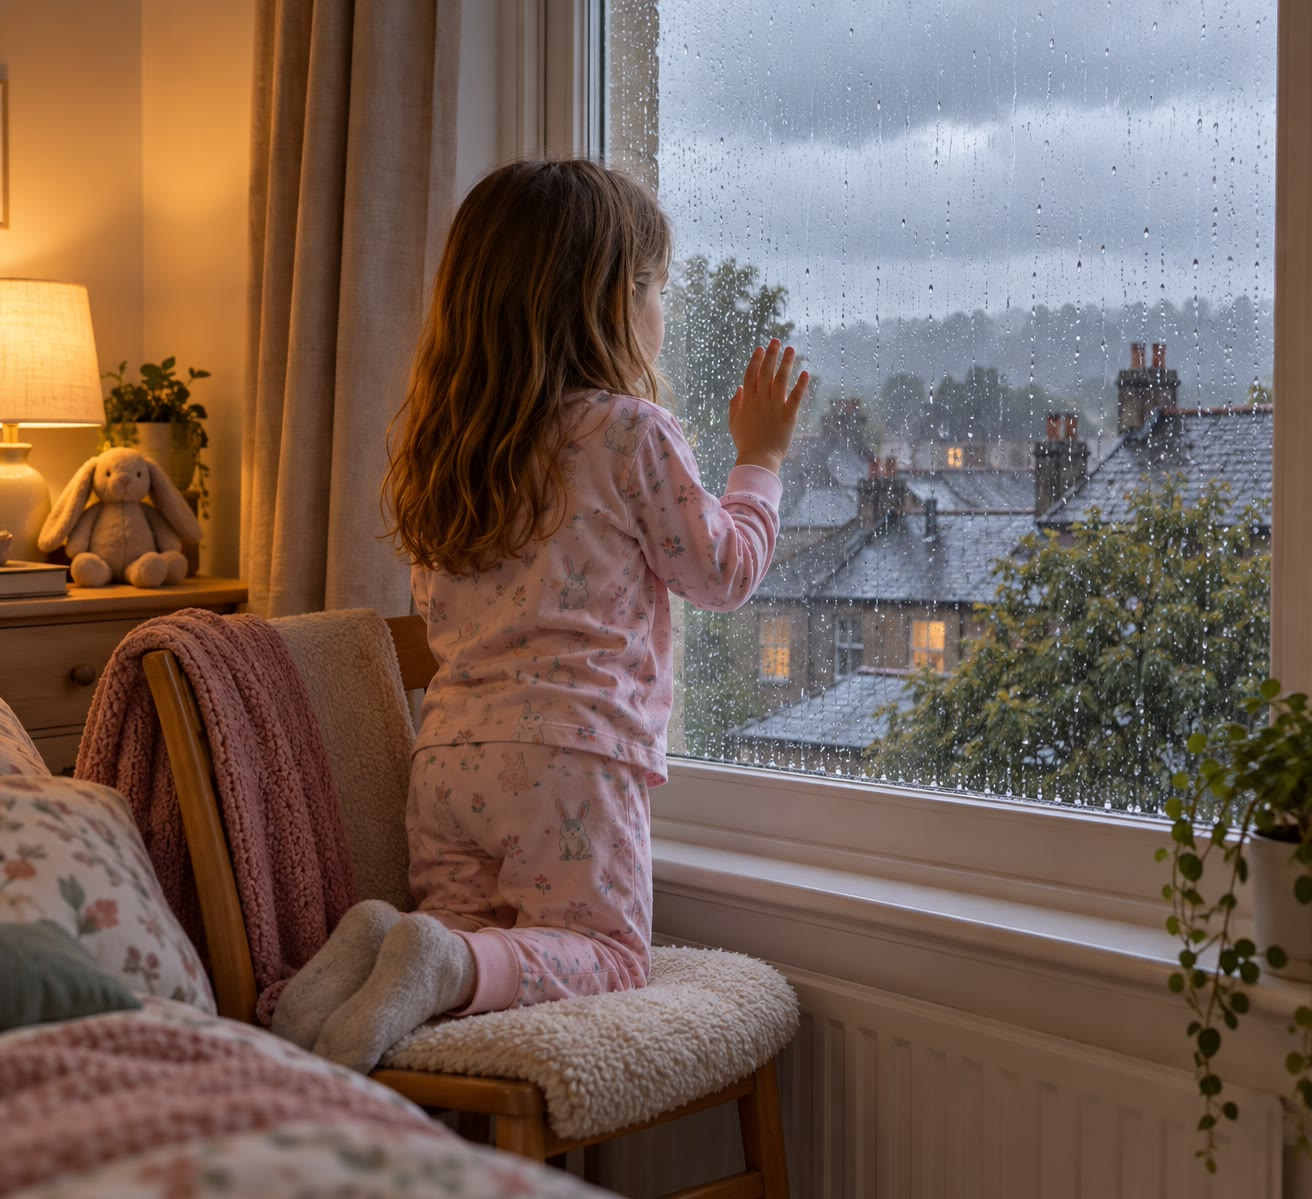
\includegraphics[width=0.72\linewidth]{images/book1/ai/g1-rainy-window.jpg}

{\small 透过窗户看到的灰蒙蒙、下着雨的早晨。}
\end{omfigure}

\begin{recall}
每天太阳升起，白天开始；每天傍晚太阳落下，
夜晚随之来临。在物理课本里，你已经了解了为什么白天之后是黑夜。
在本章中，我们研究另一种时刻都在变化的东西：
\omterm{def:g1:watching-the-weather:weather}{天气}。
\end{recall}

\section{什么是天气？}

我们走到户外时，会感觉到脸上有空气。空气可能是暖的，也可能是冷的。
空气可能很平静，也可能吹动我们的头发和衣服：这时就有风了。
我们抬头看天空。天空可能蓝蓝的、亮亮的，也可能布满云。
有时云里落下雨，有时落下雪。这些加在一起，
就是\omterm{def:g1:watching-the-weather:weather}{天气}。

\begin{definition}[天气]\label{def:g1:watching-the-weather:weather}
\emph{天气}\index{天气}是指空气和天空在某一地点、某一时刻的
状况：晴朗或多云、干燥或有雨或有雪、无风或
有风、温暖或寒冷。
\end{definition}

要描述\omterm{def:g1:watching-the-weather:weather}{天气}，我们可以回答几个简单的问题：
\begin{enumerate}
  \item \textbf{天空是什么样子的？}是蓝色的，太阳在照耀吗？
        有几朵云，还是天空全是灰的？
  \item \textbf{天上有东西落下来吗？}是雨？是雪？还是什么都没有？
  \item \textbf{有风吗？}树叶在动吗？旗子
        在飘吗？
  \item \textbf{\omterm{def:g1:watching-the-weather:weather}{天气}是暖和还是寒冷？}我们需要穿外套吗？
\end{enumerate}

\begin{omfigure}
\begin{minipage}[b]{0.49\linewidth}\centering
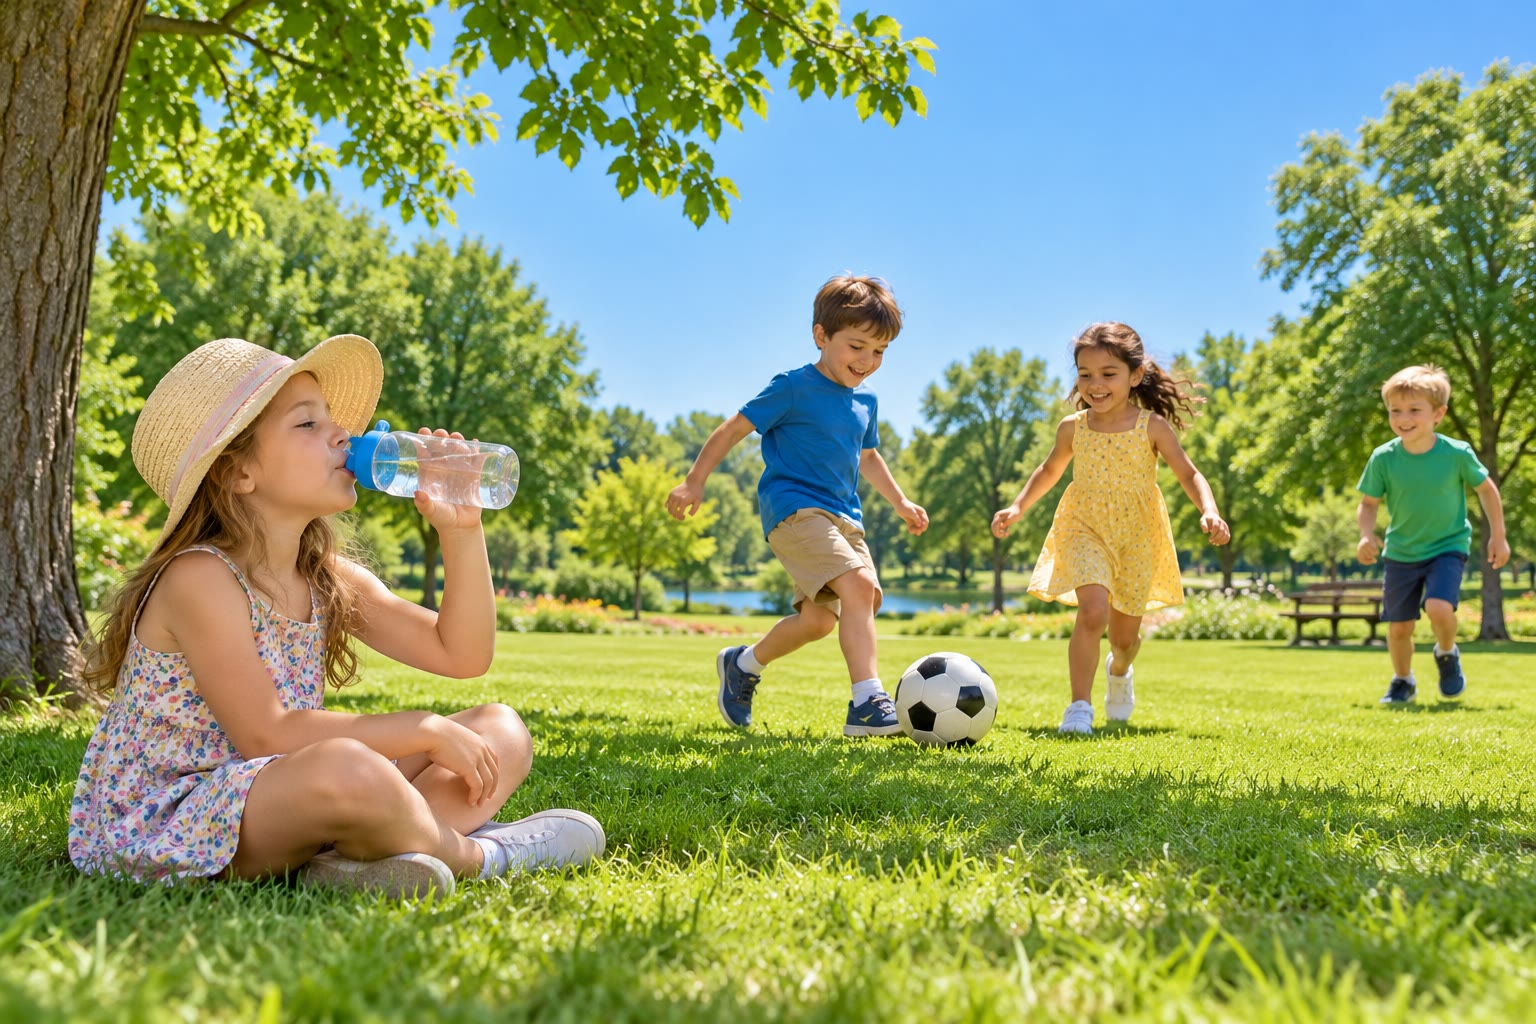
\includegraphics[width=\linewidth]{images/book1/ai/g1-sunny-park.jpg}

{\small 晴朗而温暖。}
\end{minipage}\hfill
\begin{minipage}[b]{0.49\linewidth}\centering
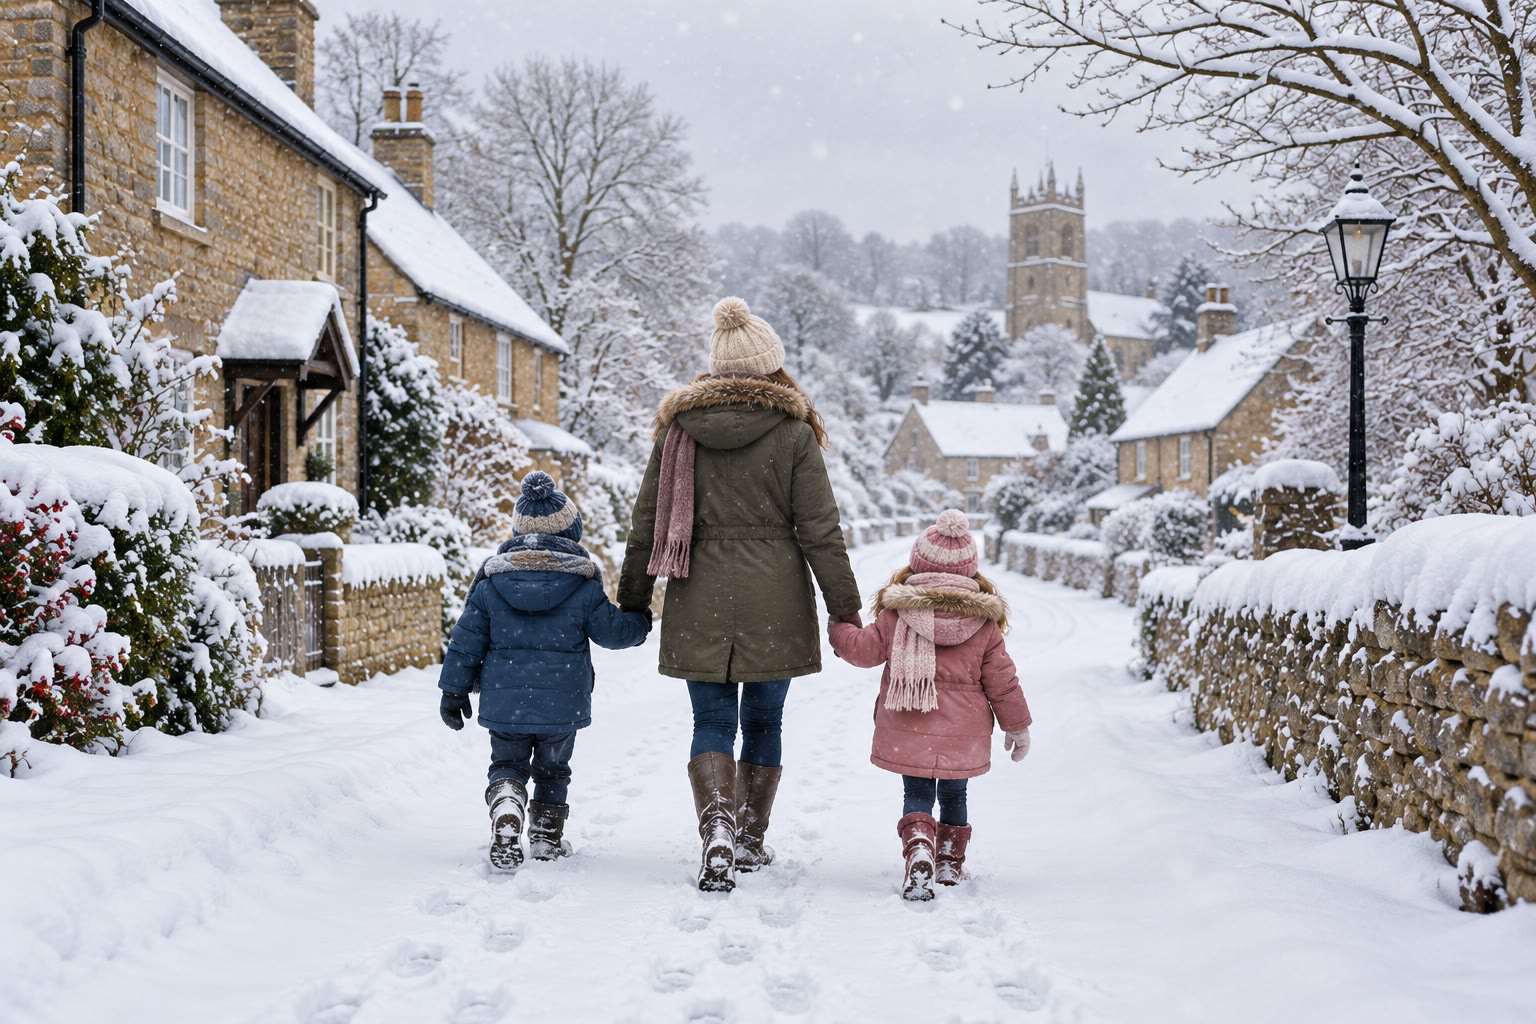
\includegraphics[width=\linewidth]{images/book1/ai/g1-snowy-street.jpg}

{\small 下雪而寒冷。}
\end{minipage}

\medskip
\begin{minipage}[b]{0.49\linewidth}\centering
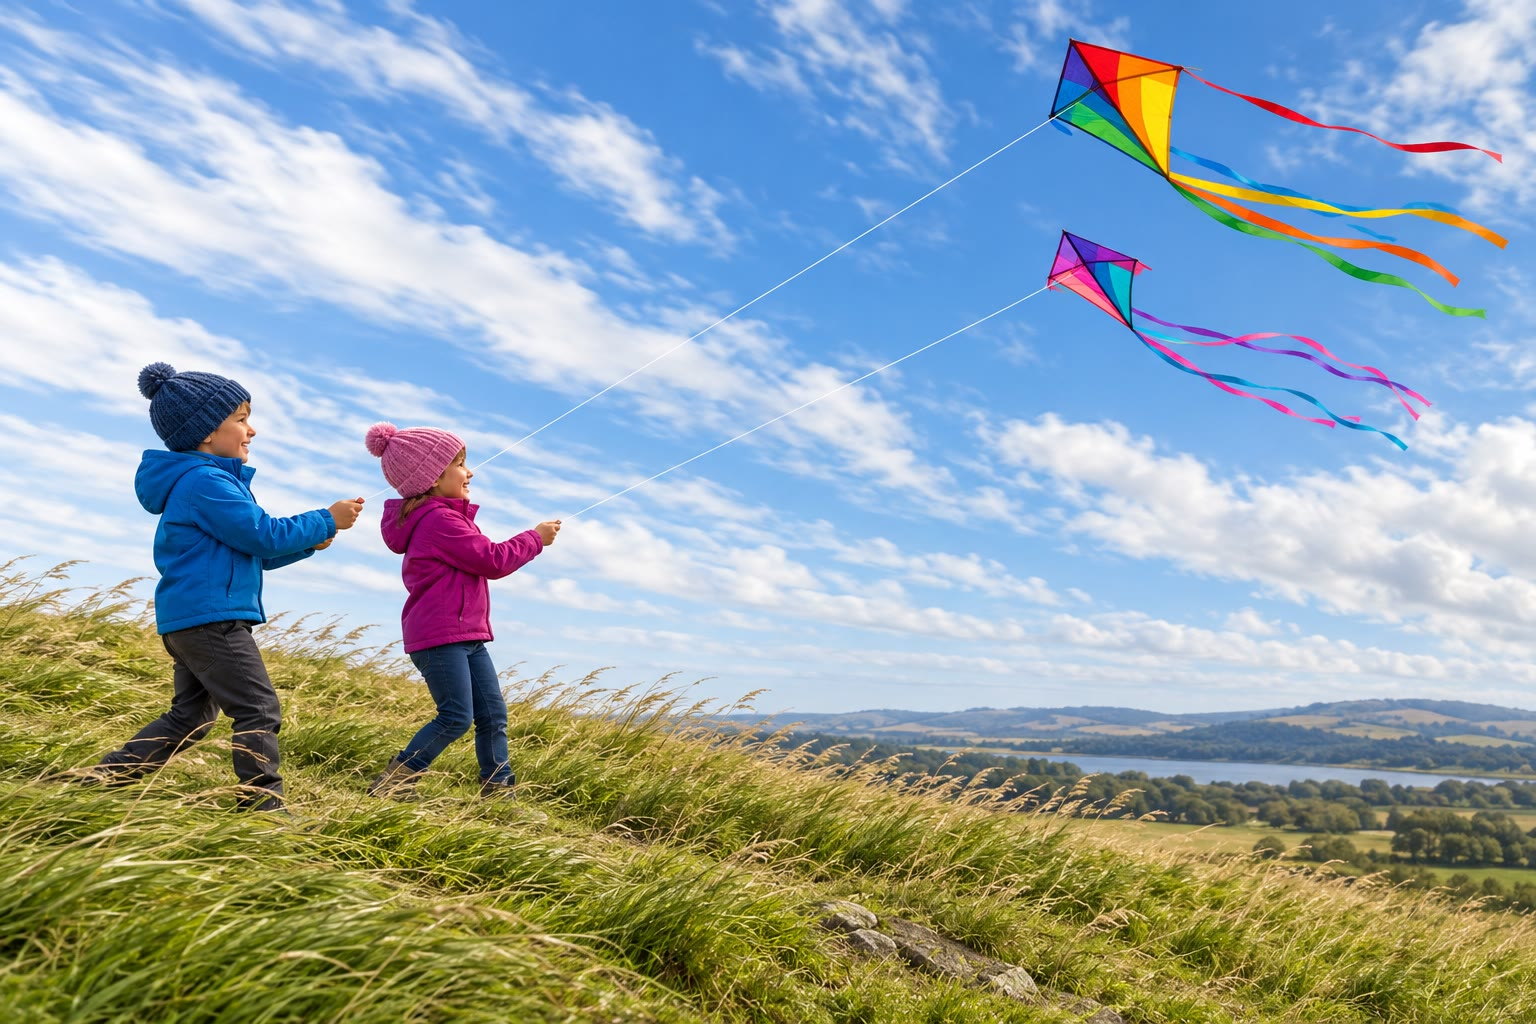
\includegraphics[width=\linewidth]{images/book1/ai/g1-windy-kites.jpg}

{\small 有风：风筝在飞。}
\end{minipage}\hfill
\begin{minipage}[b]{0.49\linewidth}\centering

\includegraphics[width=\linewidth]{images/book1/ai/g1-foggy-school.jpg}

{\small 有雾：我们看不远。}
\end{minipage}
\end{omfigure}

\begin{example}[雾]\label{ex:g1:watching-the-weather:fog}
有些早晨，空气本身看上去白茫茫的，街道尽头的
树好像消失了。这就是雾。雾是一种接触地面的云。
\omterm{def:g1:watching-the-weather:weather}{天气}变暖后，雾常常会散去。
\end{example}

\section{天气符号和天气图}

用文字描述\omterm{def:g1:watching-the-weather:weather}{天气}很费时间。观察\omterm{def:g1:watching-the-weather:weather}{天气}的人
常常改用一些小图画，也就是\omterm{def:g1:watching-the-weather:weather-chart}{天气符号}。每个符号
都容易画，也容易认。

\begin{omfigure}
\begin{tikzpicture}[x=1cm, y=1cm]
  \foreach \i/\n/\t in {0/sun/晴天, 1/suncloud/晴间多云,
      2/cloud/多云, 3/rain/雨天, 4/shower/阵雨} {
    \pic[scale=1.25, transform shape] at (\i*2.6,0) {omwx=\n};
    \node[font=\small, align=center, text width=2.4cm] at (\i*2.6,-1.05) {\t};
  }
  \foreach \i/\n/\t in {0/snow/下雪, 1/storm/雷雨, 2/fog/有雾,
      3/wind/大风} {
    \pic[scale=1.25, transform shape] at (\i*2.6+1.3,-2.6) {omwx=\n};
    \node[font=\small, align=center, text width=2.4cm] at (\i*2.6+1.3,-3.65) {\t};
  }
\end{tikzpicture}

{\small 九种\omterm{def:g1:watching-the-weather:weather-chart}{天气符号}。雷暴符号有一朵乌云，还有一道
闪电；阵雨之间会有晴朗的间歇。}
\end{omfigure}

\begin{definition}[天气图]\label{def:g1:watching-the-weather:weather-chart}
\emph{天气符号}\index{天气符号}是表示一种\omterm{def:g1:watching-the-weather:weather}{天气}的
小图画。\emph{天气图}\index{天气图}是一张表格，
我们在其中逐日记下看到的\omterm{def:g1:watching-the-weather:weather}{天气}，
用\omterm{def:g1:watching-the-weather:weather}{天气}符号表示。
\end{definition}

一个班级可以用一张\omterm{def:g1:watching-the-weather:weather-chart}{天气图}记录整整一周。每天早上，还有每天下午，
都由一名儿童向外看一看，在正确的方格里画出\omterm{def:g1:watching-the-weather:weather-chart}{天气符号}。
我们还要记下是暖和还是冷。

\begin{omfigure}
\begin{tikzpicture}[x=1cm, y=1cm]
  \def\cw{1.9}
  \foreach \d [count=\i from 0] in {星期一, 星期二, 星期三, 星期四,
      星期五, 星期六, 星期日}
    \node[font=\scriptsize\bfseries] at ({1.6+\i*\cw+\cw/2},0.35) {\d};
  \node[font=\scriptsize\bfseries, anchor=east] at (1.45,-0.5) {早上};
  \node[font=\scriptsize\bfseries, anchor=east] at (1.45,-1.5) {下午};
  \node[font=\scriptsize\bfseries, anchor=east, align=right] at (1.45,-2.35) {暖和还是 \\冷？};
  \draw[black!60] (1.6,0) rectangle ({1.6+7*\cw},-2.7);
  \foreach \i in {1,...,6}
    \draw[black!60] ({1.6+\i*\cw},0.65) -- ({1.6+\i*\cw},-2.7);
  \draw[black!60] (1.6,0.65) -- ({1.6+7*\cw},0.65);
  \draw[black!60] (1.6,0.65) -- (1.6,0);
  \draw[black!60] ({1.6+7*\cw},0.65) -- ({1.6+7*\cw},0);
  \draw[black!60] (1.6,-1) -- ({1.6+7*\cw},-1);
  \draw[black!60] (1.6,-2) -- ({1.6+7*\cw},-2);
  \foreach \i/\m/\a/\w in {0/rain/rain/冷, 1/cloud/suncloud/冷,
      2/sun/sun/暖, 3/sun/suncloud/暖, 4/suncloud/shower/暖,
      5/fog/sun/暖, 6/cloud/rain/冷} {
    \pic[scale=0.8, transform shape] at ({1.6+\i*\cw+\cw/2},-0.5) {omwx=\m};
    \pic[scale=0.8, transform shape] at ({1.6+\i*\cw+\cw/2},-1.5) {omwx=\a};
    \node[font=\scriptsize] at ({1.6+\i*\cw+\cw/2},-2.35) {\w};
  }
\end{tikzpicture}

{\small 春季一周内，某班级记录的\omterm{def:g1:watching-the-weather:weather-chart}{天气图}。}
\label{fig:g1:watching-the-weather:chart}
\end{omfigure}

\begin{method}[读天气图]\label{met:g1:watching-the-weather:read}
读\omterm{def:g1:watching-the-weather:weather-chart}{天气图}的方法：
\begin{enumerate}
  \item 找到你想看的那一天所在的列；
  \item 看行：是早上还是下午；
  \item 说出符号所表示的\omterm{def:g1:watching-the-weather:weather}{天气}。
\end{enumerate}
要数出有几天是晴天，用手指沿一行移动，
数一数太阳符号。
\end{method}

\begin{example}[读班级天气图]\label{ex:g1:watching-the-weather:read}
在本班的\omterm{def:g1:watching-the-weather:weather-chart}{天气图}上，星期一早上下雨，\omterm{def:g1:watching-the-weather:weather}{天气}寒冷。
星期三整天是晴天。星期六早上有雾，
下午转为阳光。这一周的早上，班级画太阳符号的
日子有 2 天：星期三和星期四。
\end{example}

\section{天气的变化}

\omterm{def:g1:watching-the-weather:weather}{天气}并不是一成不变的。它会在一天之内变化，从这一天到
下一天，也会在一年中变化。

\begin{itemize}
  \item \textbf{一天之内。}灰蒙蒙的早晨可以变成晴朗的
        下午。晴朗蔚蓝的早晨也可能以风暴收尾。清晨
        和夜里通常比下午更凉。
  \item \textbf{从这一天到下一天。}看看班级的\omterm{def:g1:watching-the-weather:weather-chart}{天气图}：
        本周没有任何两天完全相同。
  \item \textbf{一年之中。}夏天的日子通常暖和，而
        冬天通常寒冷；在许多地方，雪只在
        冬天下。物理书会解释季节为何
        每年都会周而复始地出现。
\end{itemize}

\begin{omfigure}
\begin{tikzpicture}[x=1cm, y=1cm]
  \draw[black!50, line width=0.8pt, -{Stealth[length=2.5mm]}] (0,0) -- (12.2,0);
  \foreach \x/\n/\t/\h in {0.9/fog/清晨/凉爽, 3.5/suncloud/上午/温和,
      6.1/sun/下午/温暖, 8.7/storm/傍晚/{温暖，有雷雨},
      11.2/suncloud/晚上/较凉} {
    \pic[scale=1.1, transform shape] at (\x,0.85) {omwx=\n};
    \fill[black!60] (\x,0) circle (1.5pt);
    \node[font=\scriptsize\bfseries, below] at (\x,-0.12) {\t};
    \node[font=\scriptsize, below] at (\x,-0.5) {\h};
  }
\end{tikzpicture}

{\small 夏天的一天，从早上到晚上：\omterm{def:g1:watching-the-weather:weather}{天气}
变化了五次。}
\label{fig:g1:watching-the-weather:day}
\end{omfigure}

\begin{omfigure}
\begin{tikzpicture}[x=1cm, y=1cm]
  \foreach \i/\s/\c/\g/\w/\gr in {0/春天/green!55!black/pink!60/suncloud/green!35,
      1/夏天/green!45!black/green!50!black/sun/green!35,
      2/秋天/orange!80!black/orange!70/rain/green!25!brown!30,
      3/冬天/black!55/white/snow/white} {
    \begin{scope}[shift={(\i*3.15,0)}]
      \draw[black!30, rounded corners=3pt, fill=ocBlue!6] (-1.4,-0.45) rectangle (1.4,3.05);
      \fill[\gr] (-1.4,-0.45) rectangle (1.4,0);
      \draw[black!25] (-1.4,0) -- (1.4,0);
      \fill[brown!60!black] (-0.09,0) rectangle (0.09,1.0);
      \draw[brown!60!black, line width=1.6pt] (0,0.75) -- (-0.5,1.35);
      \draw[brown!60!black, line width=1.6pt] (0,0.9) -- (0.45,1.45);
      \ifnum\i<3
        \fill[\c, opacity=0.85] (0,1.55) circle (0.72);
        \ifnum\i=0 \foreach \a in {20,80,140,200,260,320} \fill[\g] (0,1.55) ++(\a:0.45) circle (0.09); \fi
        \ifnum\i=2 \foreach \x/\y in {-0.9/0.15,0.7/0.3,0.95/0.1} \fill[\g] (\x,\y) circle (0.07); \fi
      \else
        \draw[white, line width=2.4pt] (-0.5,1.35) -- (-0.35,1.17);
        \draw[white, line width=2.4pt] (0.45,1.45) -- (0.3,1.27);
      \fi
      \pic[scale=0.8, transform shape] at (0.95,2.55) {omwx=\w};
      \node[font=\small\bfseries] at (0,-0.75) {\s};
    \end{scope}
  }
\end{tikzpicture}

{\small 同一棵树在四季的样子：
春天开花，夏天枝叶浓密、呈绿色，
秋天叶子变成橙色并飘落，冬天枝条光秃，挂着积雪。}
\label{fig:g1:watching-the-weather:seasons}
\end{omfigure}

\begin{remark}[风从哪里来]\label{rem:g1:watching-the-weather:wind}
我们看不见风，但能看见风的作用：旗子、风向袋
或烟囱里冒出的烟都会被风吹动，它们指向风吹去的方向，
因此风是从另一侧吹来的。
\end{remark}

\begin{omfigure}
\begin{tikzpicture}[x=1cm, y=1cm]
  % ground
  \fill[green!30!omLithAlluv] (-0.4,-0.1) rectangle (8.4,0);
  % windsock on a pole
  \draw[black!70, line width=1.2pt] (1,0) -- (1,3.2);
  \fill[orange!85, draw=black!60] (1,3.15) -- (3.4,2.95) -- (3.4,2.55) -- (1,2.45) -- cycle;
  \fill[white] (1.6,3.1) -- (2.2,3.05) -- (2.2,2.5) -- (1.6,2.47) -- cycle;
  \fill[white] (2.8,3.0) -- (3.4,2.95) -- (3.4,2.55) -- (2.8,2.53) -- cycle;
  \draw[black!60] (1,3.15) -- (3.4,2.95) -- (3.4,2.55) -- (1,2.45);
  % flag
  \draw[black!70, line width=1.2pt] (5.4,0) -- (5.4,3.2);
  \fill[ocBlue!70, draw=black!60] (5.4,3.15) .. controls (6.0,3.3) and (6.4,2.9) .. (7.1,3.05)
     -- (7.1,2.35) .. controls (6.4,2.2) and (6.0,2.6) .. (5.4,2.45) -- cycle;
  % wind arrows
  \foreach \y in {1.0,1.6}
    \draw[omWxRain, line width=1.4pt, -{Stealth[length=3mm]}] (-0.3,\y) -- (0.7,\y);
  \node[font=\small, align=right, anchor=east] at (-0.45,1.3) {风 \\从这里吹来};
  \draw[black!60, -{Stealth[length=2mm]}] (4.1,2.75) -- (4.9,2.75);
  \node[font=\small, align=left, anchor=west] at (7.5,2.7) {旗子和风向袋 \\指向 \\风吹去的方向};
\end{tikzpicture}

{\small 有风的日子里的风向袋和旗子。风从左边
吹向右边。}
\end{omfigure}

\section{我们为什么要观察天气？}

很多人需要知道\omterm{def:g1:watching-the-weather:weather}{天气}会怎样。
\begin{itemize}
  \item \textbf{农民}在割草前要看天色：雨水会毁掉干草。春天，
        他们担心降霜的夜晚，
        会冻死幼小的植物。
  \item \textbf{水手和渔民}要留意风：强风会掀起大浪，
        船只只能停留在港口。
  \item \textbf{飞行员}起飞前需要了解
        雾、风暴和风的情况。
  \item \textbf{一个班级}去森林郊游，
        想知道该带雨衣还是遮阳帽。
\end{itemize}
每天，被称为气象学家的人们观测世界各地的\omterm{def:g1:watching-the-weather:weather}{天气}，
通过广播、电视或电话告诉我们，
未来几天\omterm{def:g1:watching-the-weather:weather}{天气}可能会是怎样的。

\begin{example}[天空的征兆]\label{ex:g1:watching-the-weather:signs}
很久以前，还没有收音机和手机，人们就学会了看天空。当小小的
白云在午后长成高高的深色云塔，
就快要有阵雨或雷暴了。风向转变，天空慢慢被一层灰色薄纱覆盖时，
往往几个小时后就会下雨。
这些迹象并不总是准确，但常常很有用。
\end{example}

\section{根据天气穿衣}

现在，莉娜可以回答她的问题了。外面在下雨，\omterm{def:g1:watching-the-weather:weather}{天气}又冷，
所以她要穿上雨衣和靴子。明天\omterm{def:g1:watching-the-weather:weather}{天气}可能会不一样，
她会再重新选择。

\begin{omfigure}
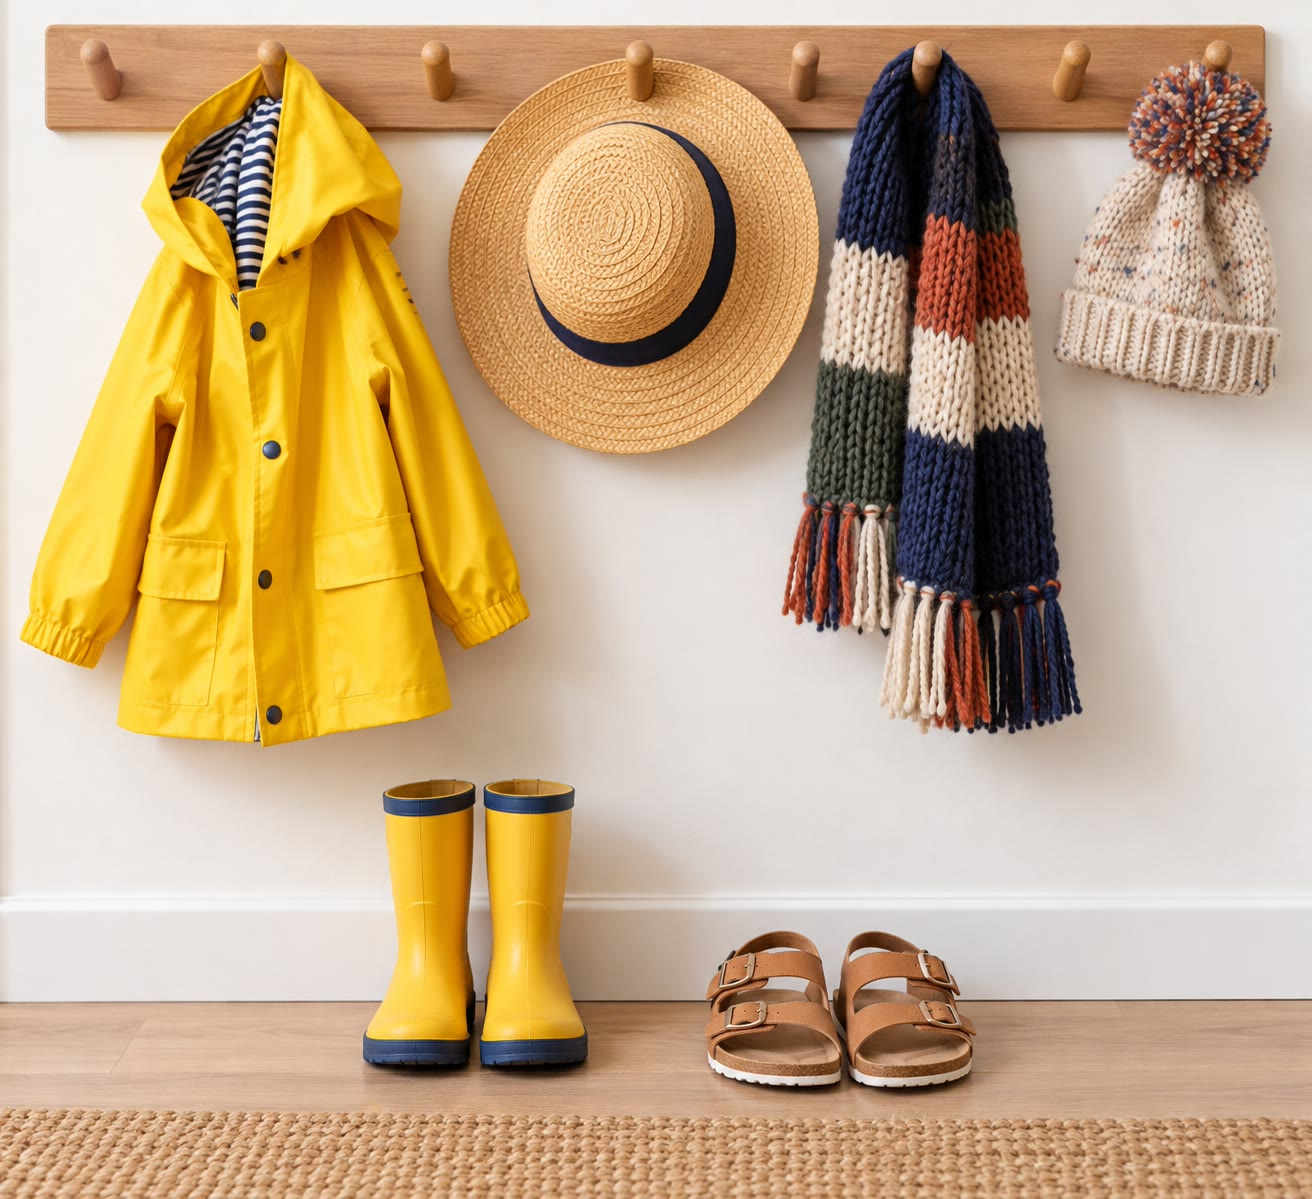
\includegraphics[width=0.66\linewidth]{images/book1/ai/g1-coat-pegs.jpg}

{\small 适合各种\omterm{def:g1:watching-the-weather:weather}{天气}的衣物：雨衣、遮阳帽、围巾
和保暖帽、靴子和凉鞋。}
\end{omfigure}

\begin{method}[根据天气选择衣物]\label{met:g1:watching-the-weather:clothes}
看看天空，感受一下空气，然后：
\begin{itemize}
  \item 下雨或有阵雨：穿雨衣或带雨伞，并穿靴子；
  \item 寒冷或下雪：穿保暖外套，戴围巾、帽子和手套；
  \item 阳光强烈、\omterm{def:g1:watching-the-weather:weather}{天气}炎热：戴遮阳帽、穿轻薄衣服，
        并带上饮用水；
  \item 有风：穿一件扣得紧的外套；雨伞帮不上多少忙。
\end{itemize}
\end{method}

\begin{safety}
\textbf{千万不要直视太阳}，哪怕一瞬间也不行，更不要
透过眼镜、双筒望远镜或照相机去看：这会永久损伤眼睛。
遇到雷暴时，待在室内或车内，远离高大的树木和水边，
等雷暴过去后再出来。
\end{safety}

\section{练习}

\begin{exercise}[$\star$]\label{exo:g1:watching-the-weather:1}
画出每种\omterm{def:g1:watching-the-weather:weather}{天气}的符号：晴、雨、雪、多云。
\end{exercise}

\begin{exercise}[$\star$]\label{exo:g1:watching-the-weather:2}
在“什么是\omterm{def:g1:watching-the-weather:weather}{天气}？”一节的四幅图中，\omterm{def:g1:watching-the-weather:weather}{天气}分别是怎样的？
每幅图用一两个词回答。
\end{exercise}

\begin{exercise}[$\star$]\label{exo:g1:watching-the-weather:3}
看看班级的\omterm{def:g1:watching-the-weather:weather-chart}{天气图}，星期二上午是什么\omterm{def:g1:watching-the-weather:weather}{天气}？
星期五下午呢？星期日下午呢？
\end{exercise}

\begin{exercise}[$\star$]\label{exo:g1:watching-the-weather:4}
在班级\omterm{def:g1:watching-the-weather:weather-chart}{天气图}上，哪一天
上午和下午都是晴天？
\end{exercise}

\begin{exercise}[$\star$]\label{exo:g1:watching-the-weather:5}
把每件衣物与一种\omterm{def:g1:watching-the-weather:weather}{天气}配对：遮阳帽；靴子和
雨衣；围巾和手套。\omterm{def:g1:watching-the-weather:weather}{天气}分别是：寒冷有雪；
炎热晴朗；下雨。
\end{exercise}

\begin{exercise}[$\star$]\label{exo:g1:watching-the-weather:6}
莉娜说：“快看，旗子在飘动！”这是什么\omterm{def:g1:watching-the-weather:weather}{天气}？
\end{exercise}

\begin{exercise}[$\star$]\label{exo:g1:watching-the-weather:7}
判断对错，并说明理由。
\begin{enumerate}
  \item 上午和下午的\omterm{def:g1:watching-the-weather:weather}{天气}总是一样的。
  \item 雾是接触地面的云。
  \item “永远不要直视太阳，即使只用一只眼睛”是一条好规则。
\end{enumerate}
\end{exercise}

\begin{exercise}[$\star\star$]\label{exo:g1:watching-the-weather:8}
在班级\omterm{def:g1:watching-the-weather:weather-chart}{天气图}上，数一数有雨或阵雨的下午有几个。
数一数寒冷的日子有几天。这一周大多是温暖还是寒冷？
\end{exercise}

\begin{exercise}[$\star\star$]\label{exo:g1:watching-the-weather:9}
萨姆一天中从窗户看到的情况是：早上，灰色的天空；
午饭时，窗户上有水滴；晚上，蓝色天空，
飘着几朵云。请按正确的顺序画出三个\omterm{def:g1:watching-the-weather:weather-chart}{天气符号}。
\end{exercise}

\begin{exercise}[$\star\star$]\label{exo:g1:watching-the-weather:10}
在风向袋和旗子的图片中，风从左侧吹来。
另一天，旗子指向左侧。那天风从哪一侧
吹来？
\end{exercise}

\begin{exercise}[$\star\star$]\label{exo:g1:watching-the-weather:11}
看看同一棵树在四个季节的图画。树在哪个季节没有叶子？
哪个季节树上有花？
冬季画的是哪个\omterm{def:g1:watching-the-weather:weather-chart}{天气符号}？它为什么适合这个季节？
\end{exercise}
